%%%%%%%%%%%%%%%%%%%%%%%%%%%%%%%%%%%%%%%%%%%%%%%%%%%%%%%%%%%%%%%%
%%                                                            %%
%%   essentialsOfLatin, Italian translation 2017              %%
%%                                                            %%
%% From:  Henry C. Pearson, Essentials Of Latin For Beginners %%
%%        (1915, New York, American Book Company)             %%
%%                                                            %%
%%    https://archive.org/details/essentialslatin04peargoog   %%
%%                                                            %%
%% Translated by g.p.ciceri <gp.ciceri@gmail.com>             %%
%% ---------------------------------------------------------- %%
%% This translation is Licensed under                         %%
%% Creative Commons Attribution-ShareAlike 4.0 International  %%
%% https://creativecommons.org/licenses/by-sa/4.0/            %%
%%                                                            %%
%%%%%%%%%%%%%%%%%%%%%%%%%%%%%%%%%%%%%%%%%%%%%%%%%%%%%%%%%%%%%%%%

% āēīōū
% ăĕĭŏŭ




\documentclass[nols]{tufte-handout}

%\geometry{showframe} % display margins for debugging page layout

\usepackage{fontspec}
\usepackage{ifxetex}
\setmainfont[Path=./fonts/palatino-linotype/, ItalicFont=palai.ttf, BoldFont=palab.ttf]{pala.ttf}


% \defaultfontfeatures{Mapping=tex-text}
% \setromanfont[Path=./fonts/TeX-Gyre-Schola/,Mapping=tex-text]{TeX Gyre Schola}
% \setsansfont[Path=./fonts/TeX-Gyre-Heros/,Scale=MatchLowercase,Mapping=tex-text]{TeX Gyre Heros}
% \setmonofont[Path=./fonts/TeX-Gyre-Cursor/,Scale=MatchLowercase]{TeX Gyre Cursor}

\usepackage{lipsum}
\usepackage{url}
\usepackage{longtable}
\usepackage{stackengine}

\usepackage{graphicx} % allow embedded images
  \setkeys{Gin}{width=\linewidth,totalheight=\textheight,keepaspectratio}
  \graphicspath{{graphics/}} % set of paths to search for images
\usepackage{amsmath}  % extended mathematics
\usepackage{booktabs} % book-quality tables
\usepackage{units}    % non-stacked fractions and better unit spacing
\usepackage{multicol} % multiple column layout facilities
\usepackage{lipsum}   % filler text
\usepackage{fancyvrb} % extended verbatim environments
  \fvset{fontsize=\normalsize}% default font size for fancy-verbatim environments

% Standardize command font styles and environments
\newcommand{\doccmd}[1]{\texttt{\textbackslash#1}}% command name -- adds backslash automatically
\newcommand{\docopt}[1]{\ensuremath{\langle}\textrm{\textit{#1}}\ensuremath{\rangle}}% optional command argument
\newcommand{\docarg}[1]{\textrm{\textit{#1}}}% (required) command argument
\newcommand{\docenv}[1]{\textsf{#1}}% environment name
\newcommand{\docpkg}[1]{\texttt{#1}}% package name
\newcommand{\doccls}[1]{\texttt{#1}}% document class name
\newcommand{\docclsopt}[1]{\texttt{#1}}% document class option name
\newenvironment{docspec}{\begin{quote}\noindent}{\end{quote}}% command specification environment

% concetti morfosintattici
\usepackage{xspace} 
\newcommand{\noun}{\textsc{sostantivo}\xspace}
\newcommand{\nouns}{\textsc{sostantivi}\xspace}
\newcommand{\adject}{\textsc{aggettivo}\xspace}
\newcommand{\adjects}{\textsc{aggettivi}\xspace}
\newcommand{\gnumber}{\textsc{numero}\xspace}
\newcommand{\gnumbers}{\textsc{numeri}\xspace}
\newcommand{\gender}{\textsc{genere}\xspace}
\newcommand{\genders}{\textsc{generi}\xspace}
\newcommand{\gcase}{\textsc{caso}\xspace}
\newcommand{\gcases}{\textsc{casi}\xspace}
\newcommand{\tense}{\textsc{tempo}\xspace}
\newcommand{\mood}{\textsc{modo}\xspace}
\newcommand{\gverb}{\textsc{verbo}\xspace}
\newcommand{\gverbs}{\textsc{verbi}\xspace}
\newcommand{\adjective}{\textsc{aggettivo}\xspace}
\newcommand{\nom}{\textsc{nom}\xspace}
\newcommand{\gen}{\textsc{gen}\xspace}
\newcommand{\dat}{\textsc{dat}\xspace}
\newcommand{\acc}{\textsc{acc}\xspace}
\newcommand{\voc}{\textsc{voc}\xspace}
\newcommand{\abl}{\textsc{abl}\xspace}
\newcommand{\gexit}{\textsc{uscita}\xspace}
\newcommand{\gexits}{\textsc{uscite}\xspace}
\newcommand{\declinazione}{\textsc{declinazione}\xspace}
\newcommand{\masc}{\textsc{maschile}\xspace}
\newcommand{\femm}{\textsc{femminile}\xspace}
\newcommand{\neut}{\textsc{neutro}\xspace}

\newcommand{\indic}{\textsc{indicativo}\xspace}
\newcommand{\imper}{\textsc{imperativo}\xspace}
\newcommand{\gcong}{\textsc{congiuntivo}\xspace}
\newcommand{\ott}{\textsc{ottativo}\xspace}
\newcommand{\partic}{\textsc{participio}\xspace}
\newcommand{\infin}{\textsc{infinito}\xspace}

\newcommand{\pres}{\textsc{presente}\xspace}
\newcommand{\imperf}{\textsc{imperfetto}\xspace}
\newcommand{\aor}{\textsc{aoristo}\xspace}
\newcommand{\fut}{\textsc{futuro}\xspace}
\newcommand{\perf}{\textsc{perfetto}\xspace}
\newcommand{\pperf}{\textsc{piuccheperfetto}\xspace}

\newcommand{\sing}{\textsc{singolare}\xspace}
\newcommand{\plur}{\textsc{plurale}\xspace}
\newcommand{\dual}{\textsc{duale}\xspace}

\newcommand{\si}{\textsc{sing}\xspace}
\newcommand{\pl}{\textsc{plur}\xspace}
\newcommand{\du}{\textsc{dual}\xspace}

\newcommand{\att}{\textsc{attivo}\xspace}
\newcommand{\med}{\textsc{medio}\xspace}
\newcommand{\pass}{\textsc{passivo}\xspace}
\newcommand{\medpass}{\textsc{medio-passivo}\xspace}


% italianitudini
\renewcommand{\figurename}{Figura}
\renewcommand{\tablename}{Tabella}
\renewcommand{\contentsname}{Indice}

% fix per un qualche problema
\ifxetex
  \newcommand{\textls}[2][5]{%
    \begingroup\addfontfeatures{LetterSpace=#1}#2\endgroup
  }
  \renewcommand{\allcapsspacing}[1]{\textls[15]{#1}}
  \renewcommand{\smallcapsspacing}[1]{\textls[10]{#1}}
  \renewcommand{\allcaps}[1]{\textls[15]{\MakeTextUppercase{#1}}}
  \renewcommand{\smallcaps}[1]{\smallcapsspacing{\scshape\MakeTextLowercase{#1}}}
  \renewcommand{\textsc}[1]{\smallcapsspacing{\textsmallcaps{#1}}}
\fi

% too many float...
\extrafloats{100}
% āēīōū
% ăĕĭŏŭ

\title{Essentials Of Latin. Elementi di Latino. \newline Lezione VIII - Seconda Declinazione (continua). nomi maschili in -er e -ir.}

\author[gpciceri]{a cura di Milagathòs: Milo's help to enjoy humanities.}

\date{22 Febbrajo 2017} % without \date command, current date is supplied


\begin{document}

\hyphenation{co-niu-ga-zio-ne}

\maketitle% this prints the handout title, author, and date

\begin{marginfigure}[-2.5cm]
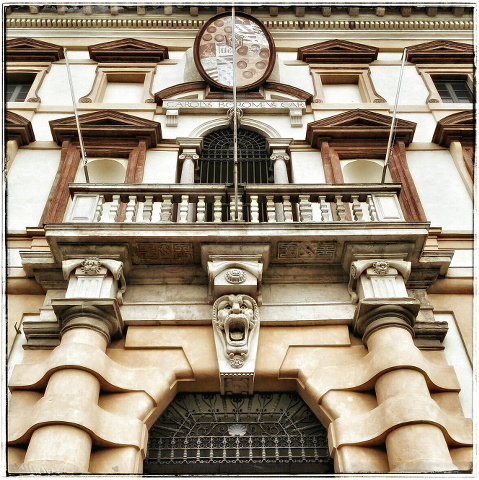
\includegraphics{smallthumb-lesson_I.jpeg}
\setfloatalignment{b}
\end{marginfigure}


\begin{abstract}
\noindent
Queste lezioni riprendono il testo introduttivo al Latino di Pearson\cite{pearson1915}, del quale seguono la numerazione; la struttura di ogni lezione è piuttosto regolare: inizia con \textsc{cenni di morfologia e di sintassi latina}, seguita da un \textsc{piccolo vocabolario} per il lessico; ci sono infine vari \textsc{esercizi} di traduzione e di composizione latina.

\bigskip
\noindent
Lezione VIII - Seconda declinazione, nomi maschili in -er e -ir, vocabolario, esercizi.
\end{abstract}

%\printclassoptions

% āēīōū
% ăĕĭŏŭ

\newthought{69. Seconda Declinazione, nomi in -er e -ir.} \textbf{puer, -ī}, \textit{ragazzo}. Radice \textbf{puero-}, tema \textbf{puer-}; 
\textbf{ager, -ī}, \textit{campo}. Radice \textbf{agro-}, tema \textbf{agr-};
\textbf{vir, -ī}, \textit{uomo}. Radice \textbf{viro-}, tema \textbf{vir-}.

\begin{fullwidth}
\begin{table}[!htbp]
  \centering
  \begin{tabular}{l l l l}
    %\toprule
	& \multicolumn{3}{c}{\textsc{Singolare}} \\

    \nom & puer            & ager           & vir  \\
    \gen & puer\textbf{ī}  & agr\textbf{ī}  & vir\textbf{ī}  \\
    \dat & puer\textbf{ō}  & agr\textbf{ō}  & vir\textbf{ō}  \\
    \acc & puer\textbf{um} & agr\textbf{um} & vir\textbf{um} \\
    \voc & puer            & ager           & vir             \\
    \abl & puer\textbf{ō}  & agr\textbf{ō}  & vir\textbf{ō}  \\
	
	\multicolumn{4}{c}{\textemdash} \\
	
	& \multicolumn{3}{c}{\textsc{Plurale}} \\
	
	\nom & puer\textbf{ī}  & agr\textbf{ī}  & vir\textbf{ī}  \\
    \gen & puer\textbf{ōrum}  & agr\textbf{ōrum}  & vir\textbf{ōrum}  \\
    \dat & puer\textbf{īs}  & agr\textbf{īs}  & vir\textbf{īs}  \\
    \acc & puer\textbf{ōs} & agr\textbf{ōs} & vir\textbf{ōs} \\
    \voc & puer\textbf{ī}  & agr\textbf{ī}  & vir\textbf{ī}   \\
    \abl & puer\textbf{īs}  & agr\textbf{īs}  & vir\textbf{īs}  \\
	
    %\bottomrule
  \end{tabular}
  %\caption[bottom]{Prima Declinazione. \textbf{stella, -ae}, f.}
  \label{tab:normaltab}
  %\zsavepos{pos:normaltab}
\end{table}
\end{fullwidth}

\begin{itemize}
\item[\textsc{1.}] Le terminazioni sono le stesse della sezione 50.?  
\item[\textsc{2.}] Il tema è formato come negli altri nomi? 
\item[\textsc{3.}] Il vocativo è uguale al nominativo.  
\item[\textsc{4.}] Confronta con cura \textbf{puer} e \textbf{ager}, osserva che il tema di \textbf{ager} perde la \textbf{e} prima della\textbf{r}.  
\end{itemize}


\newthought{70} Solo pochi nomi vengono declinati come \textbf{puer}. La maggior parte dei nomi della seconda declinazione in \textbf{-er} vengono declinati come \textbf{ager}.
\begin{itemize}
\item Declina \textbf{liber}, \textit{libro} come \textbf{ager}.  
\item Declina \textbf{liberi}, \textit{bambini}, come il plurale di \textbf{puer}.   
\end{itemize}


\newthought{71. Vocabolario} 

\begin{multicols}{2}
    \noindent \hangindent=1em \textbf{liber, librī}, m., \textit{libro}.  \\
    \noindent \hangindent=1em \textbf{liberī, līberōrum}, m.pl., \textit{bambini}.  \\
    \noindent \hangindent=1em \textbf{magister, magistrī}, m., \textit{maestro, insegnante}.  \\
    \noindent \hangindent=1em \textbf{ager, agrī}, m., \textit{campo}.  \\
    \noindent \hangindent=1em \textbf{Gallus, -ī}, m., \textit{il Gallo (abitante della Gallia)}.  \\
    \noindent \hangindent=1em \textbf{puer, puerī}, m., \textit{ragazzo}.  \\
    \noindent \hangindent=1em \textbf{discipulus, -ī}, m., \textit{alunno}.  \\
    \noindent \hangindent=1em \textbf{multus, a, um}, agg., \textit{molto}.  \\
\end{multicols}
% āēīōū
% ăĕĭŏŭ

\newthought{72. Esercizi di Ripasso}
\\
\textsc{I.} \quad
\textsc{1.}~Inopia frumenti est in Gallia. \quad
\textsc{2.}~Incolis oppidi magni equos dant. \quad
\textsc{3.}~Servus dona agricolae in oppidum portat. \quad
\textsc{4.}~Estne nunc pecuniae copia? \quad
\textsc{5.}~Agricolarum vita Gallos non delectat. \quad
\textsc{6.}~Cur in pulchram insulam frumentum portamus?
\\
\textsc{II.} \quad
\textsc{1.}~Gli abitanti gradiscono una buona storia. \quad
\textsc{2.}~Ci sono molti agricoltori nel mio paese, e robusti. \quad
\textsc{3.}~I romani radunano grandi forze (armate) nelle città. \quad
\textsc{4.}~Ci sono contadini nella foresta e molti marinai sull'isola.


\newthought{73. Esercizi}
\\
\textsc{I.} \quad
\textsc{1.}~Multi libri sunt in oppido. \quad
\textsc{2.}~Viri puellas et pueros laudant. \quad
\textsc{3.}~Cibum in oppidum portamus. \quad
\textsc{4.}~Liber meo discipulo est gratus. \quad
\textsc{5.}~Regina liberos in oppidum convocat. \quad
\textsc{6.}~Discipuli magistri amicum laudant. \quad
\textsc{7.}~Multi agricolae nonc in agro sunt. \quad
\textsc{8.}~Filia mea liberos magistri laudat. \quad
\textsc{9.}~Incolarum agri sunt lati. \quad
\textsc{10.}~Magister discipulos non semper culpat. \quad
\textsc{11.}~Ubi nunc sunt filiae meae libri? \quad
\textsc{12.}~Equi multos viros in silvam portant.
\\
\textsc{II.} \quad
\textsc{1.}~I ragazzi sono amici dei miei figli. \quad
\textsc{2.}~Mia figlia adora la sua insegnante. \quad
\textsc{3.}~I robusti contadini chiamano gli schiavi nei campi. \quad
\textsc{4.}~L'insegnante dà un libro all'uomo. \quad
\textsc{5.}~Non ci sono molti marinai in città. \quad
\textsc{6.}~L'insegnante loda i suoi alunni fedeli.


\begin{figure}[!b]
  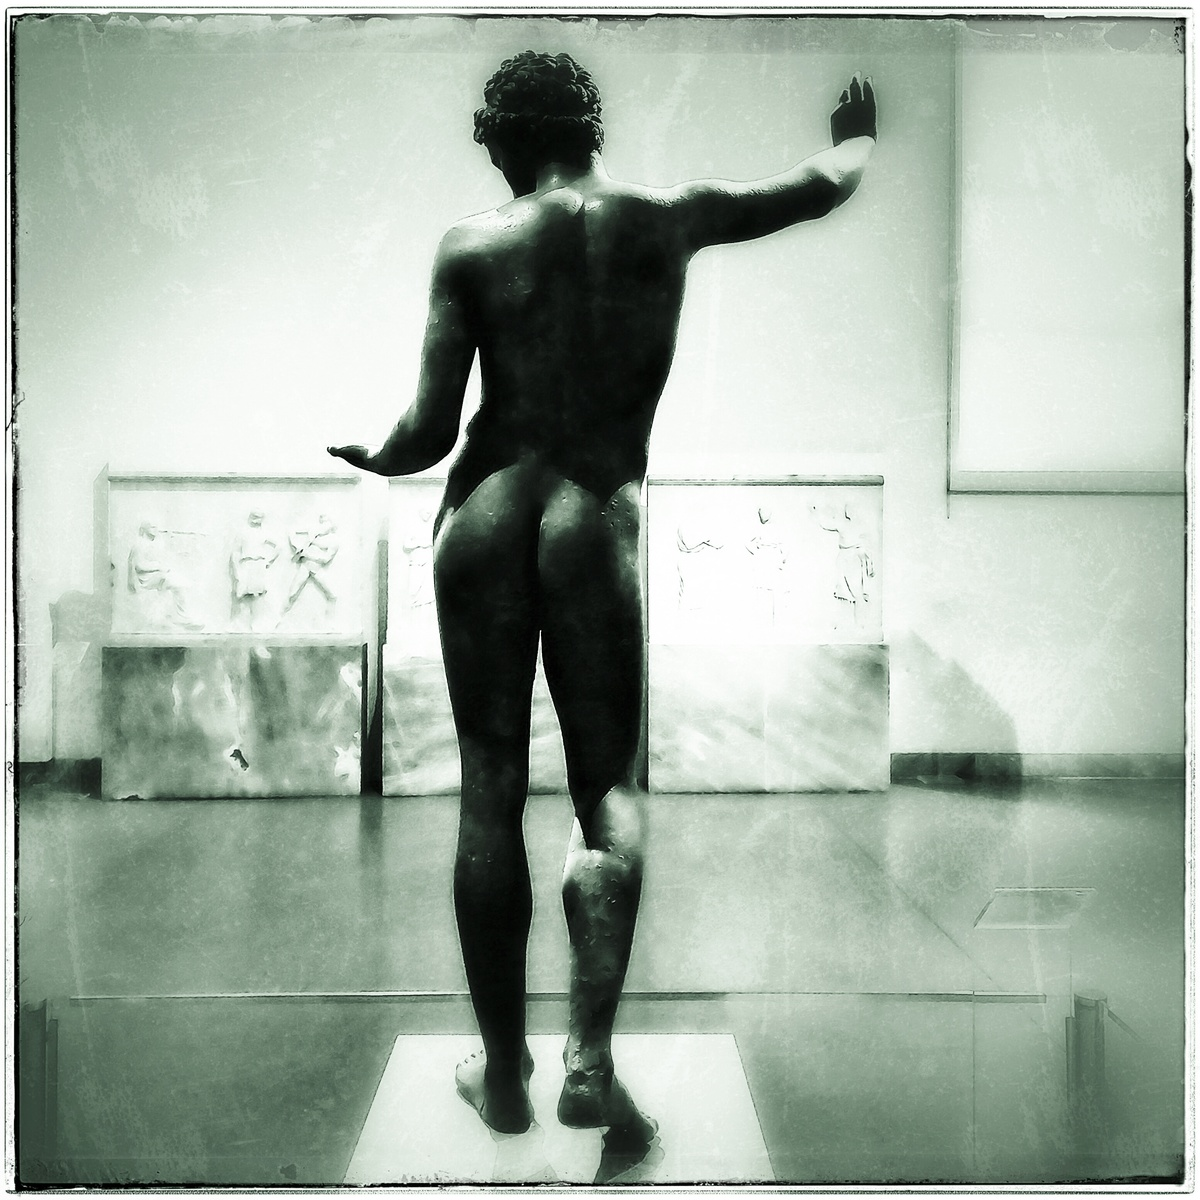
\includegraphics[width=0.8\linewidth]{thumb-lesson_VII.jpeg}
  %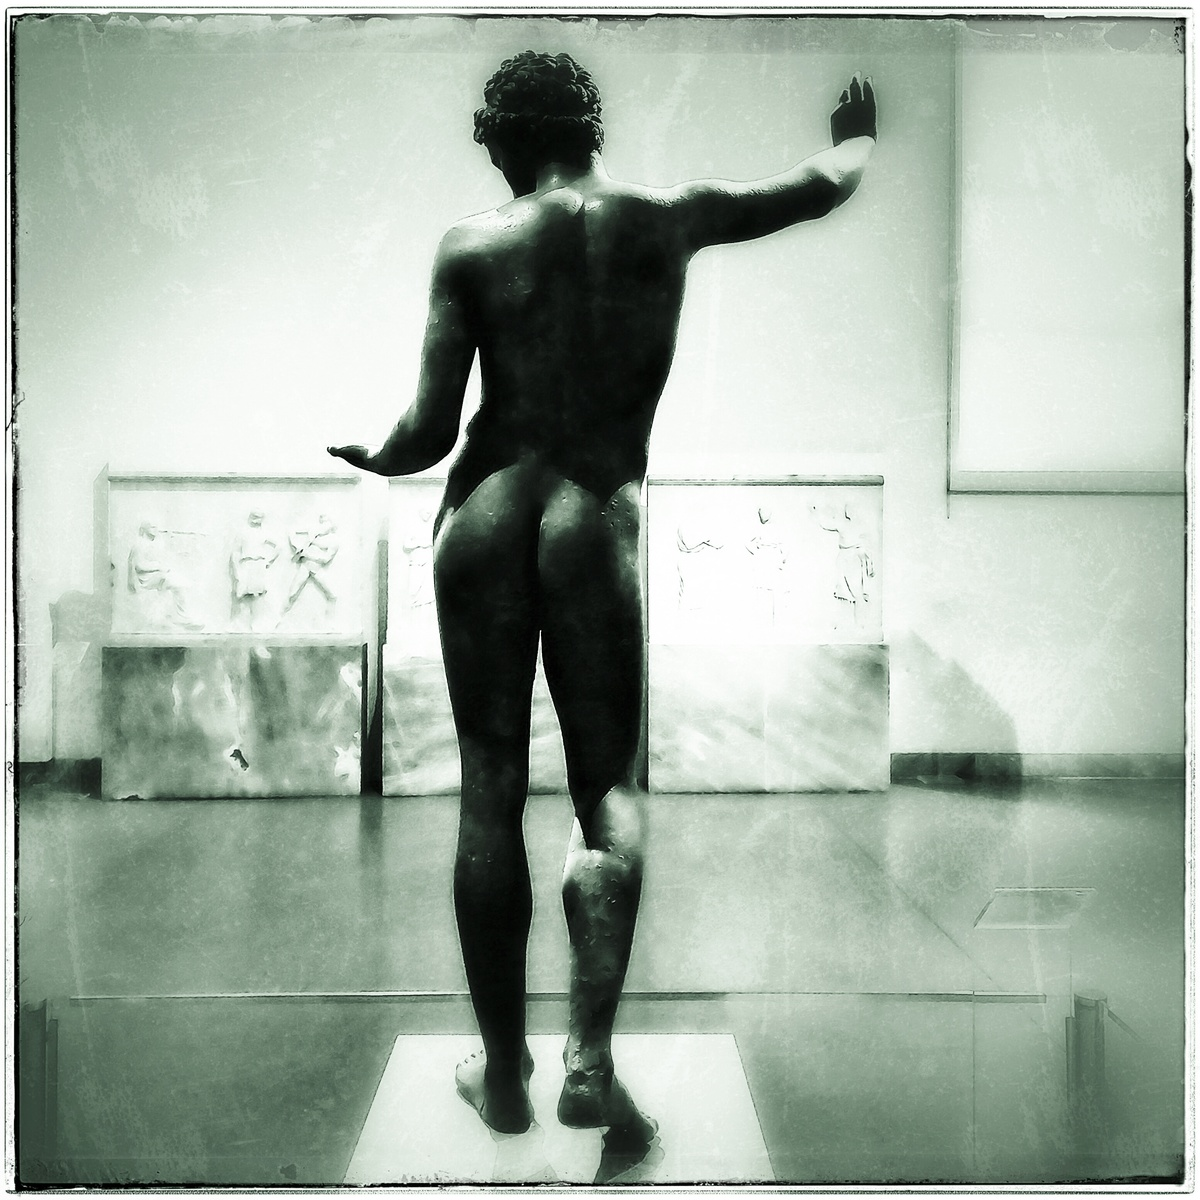
\includegraphics{thumb-lesson_VII.jpeg}
  \caption{Pavia: Almo Collegio Borromeo}
  \label{fig:textfig}
  %\zsavepos{pos:textfig}
  %\setfloatalignment{b}
\end{figure}

 

\nobibliography{latinBiblio}
\bibliographystyle{alpha}


\end{document}
